% Geometry, font
\documentclass[12pt, letter]{article}
\usepackage[margin=0.8in]{geometry}
\usepackage[T1]{fontenc}
\usepackage{fourier}
\usepackage{titling}
\setlength{\droptitle}{-5em} 
\usepackage[parfill]{parskip}
\usepackage{graphicx}
\graphicspath{{imgs/}}
\usepackage{hyperref}

% Math stuff
\usepackage{amssymb}
\usepackage{bm}

% Code Highlighting
\usepackage{minted}
\usemintedstyle{solarizedlight}

\author{Zach Neveu}
\title{ Day 11 Notes }

\begin{document}
\maketitle

\section{Agenda}%
\label{sec:agenda}
\begin{itemize}
	\item LP solving with simplex
	\item Introduction to LP
	\item Homework \#3 due Friday
	\item Quiz \#3 next Tuesday
\end{itemize}

\section{LP}%
\label{sec:lp}
Options for LP soln: \\
\begin{itemize}
	\item Single possible solution
	\item No feasible solution
	\item Unbounded feasible region
	\item Infinite optimal solutions along line segment
\end{itemize}

\begin{figure}[h]
	\centering
	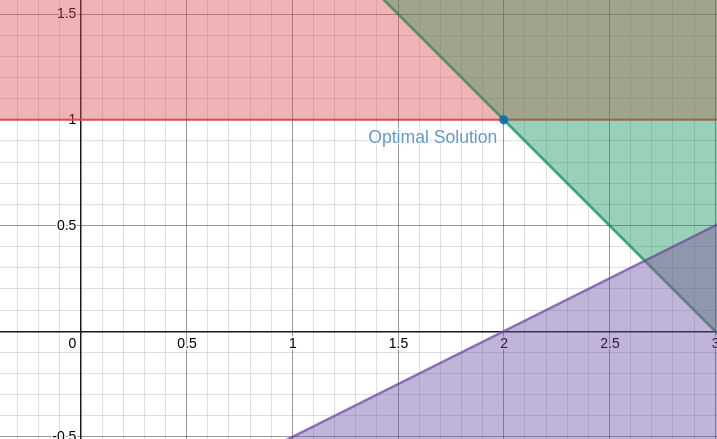
\includegraphics[width=0.8\textwidth]{single-soln}
	\caption{Single Solution}
	\label{fig:single-soln}
\end{figure}

\begin{figure}[h]
	\centering
	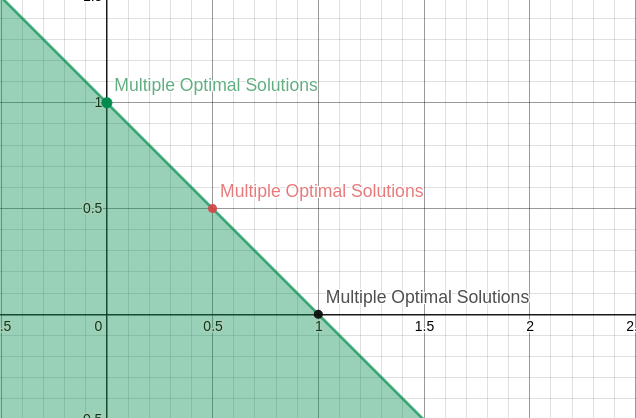
\includegraphics[width=0.8\textwidth]{mult-solns}
	\caption{Multiple Solutions Along Segment}
	\label{fig:mult-soln}
\end{figure}

\begin{figure}[h]
	\centering
	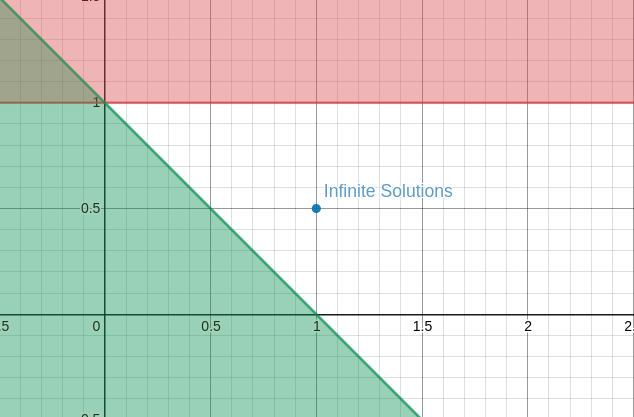
\includegraphics[width=0.8\textwidth]{inf_solns}
	\caption{Unbounded Feasible Region}
	\label{fig:inf-solns}
\end{figure}

\begin{figure}[h]
	\centering
	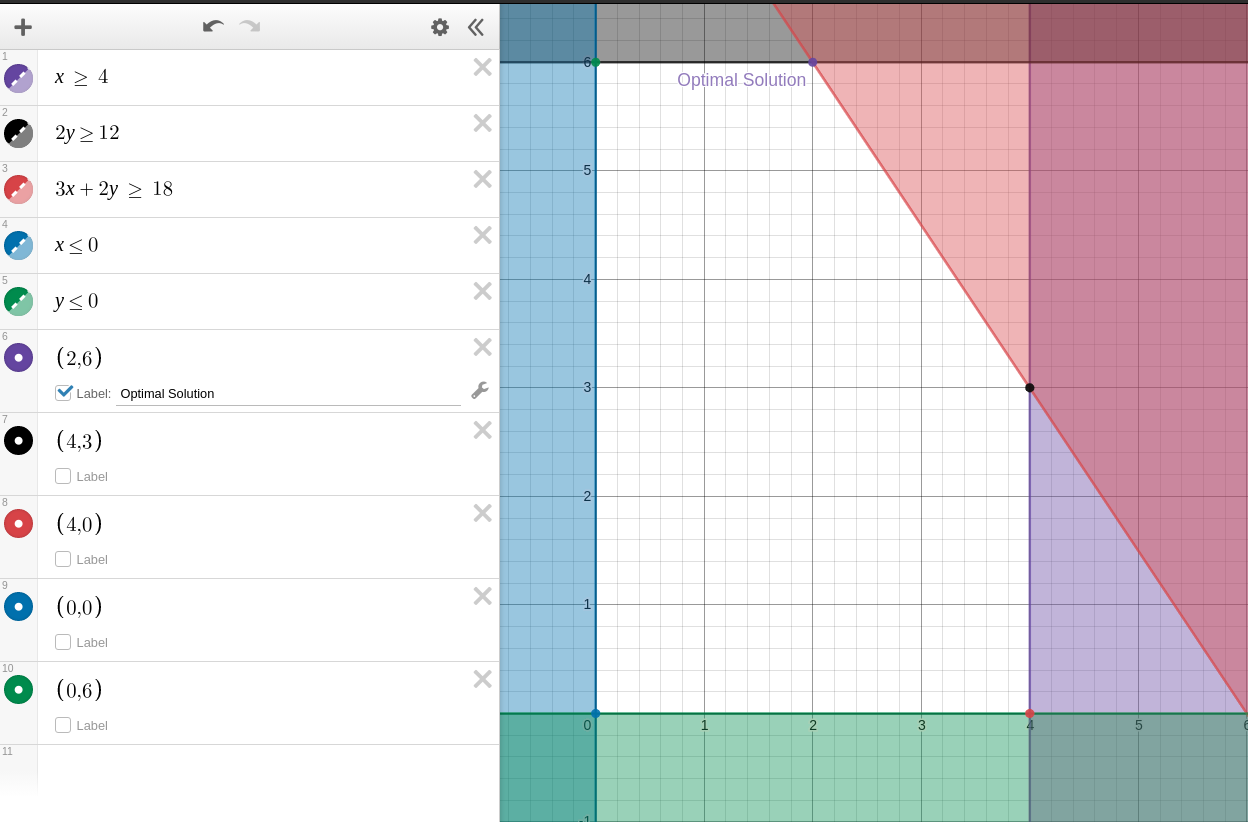
\includegraphics[width=0.8\textwidth]{textbook-lp}
	\caption{Example LP from Text Book}
	\label{fig:textbook-lp}
\end{figure}

\begin{itemize}
	\item \textbf{Cornerpoint Feasible Solution (CPF Solution):} Cornerpoint solutions that border the feasible region.
	\item Number of cornerpoints $\le {constraints \choose 2}$
	\item Adjacent CPF solutions are connected along the edge of a constraint
	\item Optimality Test: If a CPF Solution is better than all adjacent CPF solutions, then it must be optimal.
	\item This works because simplex is always \textbf{convex} 
	\item \textbf{Convex:} Lines connecting all pairs of nodes fall completely within the enclosed area
    \item \textbf{Boundary} of the feasible region is the parts of the constraint boundaries that are feasible
    \item CPF solutions in 3 dimensions are the intersection of 3 planes
    \item In 3 dimensions, each CPF solution has up to 3 possible adjacent solutions
    \item \textbf{Edge:} The feasible portion of the intersection of 2 constraint boundaries 
    \item Number of possible CPF solutions can be exponentially large (num constraints choose num dimensions)
    \item Not trivial to search through all possible CPF solutions in certain cases
    \item Bad news: Possible to create an intractable simplex instance
    \item Good news: In practice, instances are solved very fast
    \item More Good news: other algorithms can solve LP problems in P!
\end{itemize}

\subsection*{Simplex Algorithm}
\begin{enumerate}
	\item Initialization: pick an initial CPF Solution
	\item Optimality test
	\item Select new CPF Solution that is adjacent
	\item Go back to 2 until optimality test passes.
\end{enumerate}

\section{Using LP in Class}%
\label{sec:using_lp_in_class}
\begin{figure}[h]
    \centering
    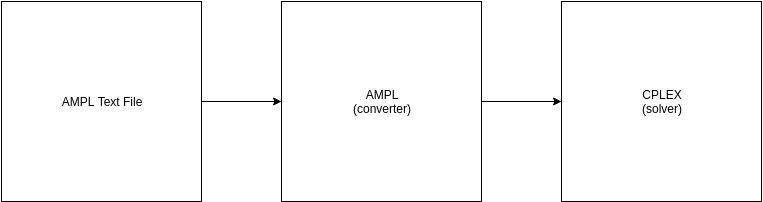
\includegraphics[width=0.8\textwidth]{solver}
    \caption{Flow Diagram of Solving Process}
    \label{fig:solver}
\end{figure}

\subsection*{AMPL Notes}

\begin{minted}{Python}
# Write in *.mod file
var x1;
var x2;
maximize objective: x1+x2;
subject to constraint1:
    4*x1-x2 <= 18;
constraint2:
    2*x1+x2 <=  18;
\end{minted}

\begin{enumerate}
    \item Write AMPL commands into *.mod file
    \item Run \texttt{ampl} at unix prompt to launch AMPL
    \item run \texttt{model *.mod} to load model
    \item run \texttt{data *.dat} to load data
    \item run \texttt{solve;}  to solve
    \item Solver spits out \# of simplex steps required
    \item run \texttt{display x1;} to display result
    \item run \texttt{include *.run} to run script of AMPL commands
    \item run \texttt{ampl *.run} from unix prompt to run script
\end{enumerate}

\subsection*{AMPL Examples}

\begin{minted}{AMPL}
param N=10;
var x {i in 0..N-1};
subject to C1:
    x[0]+3*x[i] <=  10;
c2:
    sum{i in 0..N-1} x[0] = 0;
c3 {j in 0..10}: x[j] = x[j+1];
\end{minted}

\begin{itemize}
    \item Variables $\ne$ Parameters
    \item Parameters are known at solve time - unchanging
    \item Variables: may change in execution
    \item Store params in data file
    \item Store variables in model file
\end{itemize}


\end{document}
